\section{The Solution}
\subsection{Data Preperation}
%The problem that the neural network is trained for relies on time depended data, i.e. time based weather data where the order of events
%does have an impact on the outcome. To include that, recurrent neural networks, short RNN, will be build the ground for a first approach. 
%As an eviroment to build the model in, \enquote{Keras} has been choosen as it provides all the tools, layer structures and evaluation methods 
%to tackle the problem at hand \cite{keras}. At first the dataset has to be further prepared 
%and sorted that the outcome shape will divide every city, with each city including 51 days of 8 features.
%It follows that one entry contains 51 time sequenced rows with informations. A test train split, provided by \enquote{Keras} \cite{keras}, will 
%randomly seperate the data into different regimes: 20\% test, 64\% train, 16\% validation. Each regime will be split in two, where the first 40 entires, i.e. days, of each city
%will be the input of the model and the last 11 entries of confirmed cases (shape (11,1)) the output, i.e. target.
%To handle outlier and make the sets more handable for the umpcoming network 
%a \enquote{Standardscaler} \cite{keras} will be applied to each of them.
The problem that the neural network is trained for relies on time-dependent data, i.e., time-based weather data where the order of events
has an impact on the outcome. To include that, recurrent neural networks, or RNNs for short, will be used as the foundation for a first approach.
As an environment to build the model in, \enquote{Keras} has been chosen as it provides all the tools, layer structures, and evaluation methods
to tackle the problem at hand \cite{keras}. The dataset needs to be further prepared and sorted so that the outcome shape will divide every city, with each city including 51 days of 8 features.
This means that one entry contains 51 time-sequenced rows with information. A test-train split, provided by \enquote{Keras} \cite{keras}, will
randomly separate the data into different regimes: 20\% for testing, 64\% for training, and 16\% for validation. Each regime will be split in two, where the first 40 entries, i.e. days, of each city
will be the input of the model, and the last 11 entries of confirmed cases (shape (11,1)) will be the output, i.e., the target.
To handle outliers and make the sets more manageable for the upcoming network, a \enquote{StandardScaler} \cite{keras} will be applied to each of them.

%\subsection{The Model}
%Since the already foreseen use of RNNs, three simple models have been constructed each with one layer containing:
%\enquote{SimpleRNN}, \enquote{GRU} and \enquote{LSTM} to get a quick overview on how each RNN architecture perfoms on this problem.
\subsection{The Model}
Since the already foreseen use of RNNs, three simple models have been constructed, each with one layer containing:
\enquote{SimpleRNN}, \enquote{GRU}, and \enquote{LSTM}, to get a quick overview of how each RNN architecture performs on this problem.

\begin{figure}
    \centering
    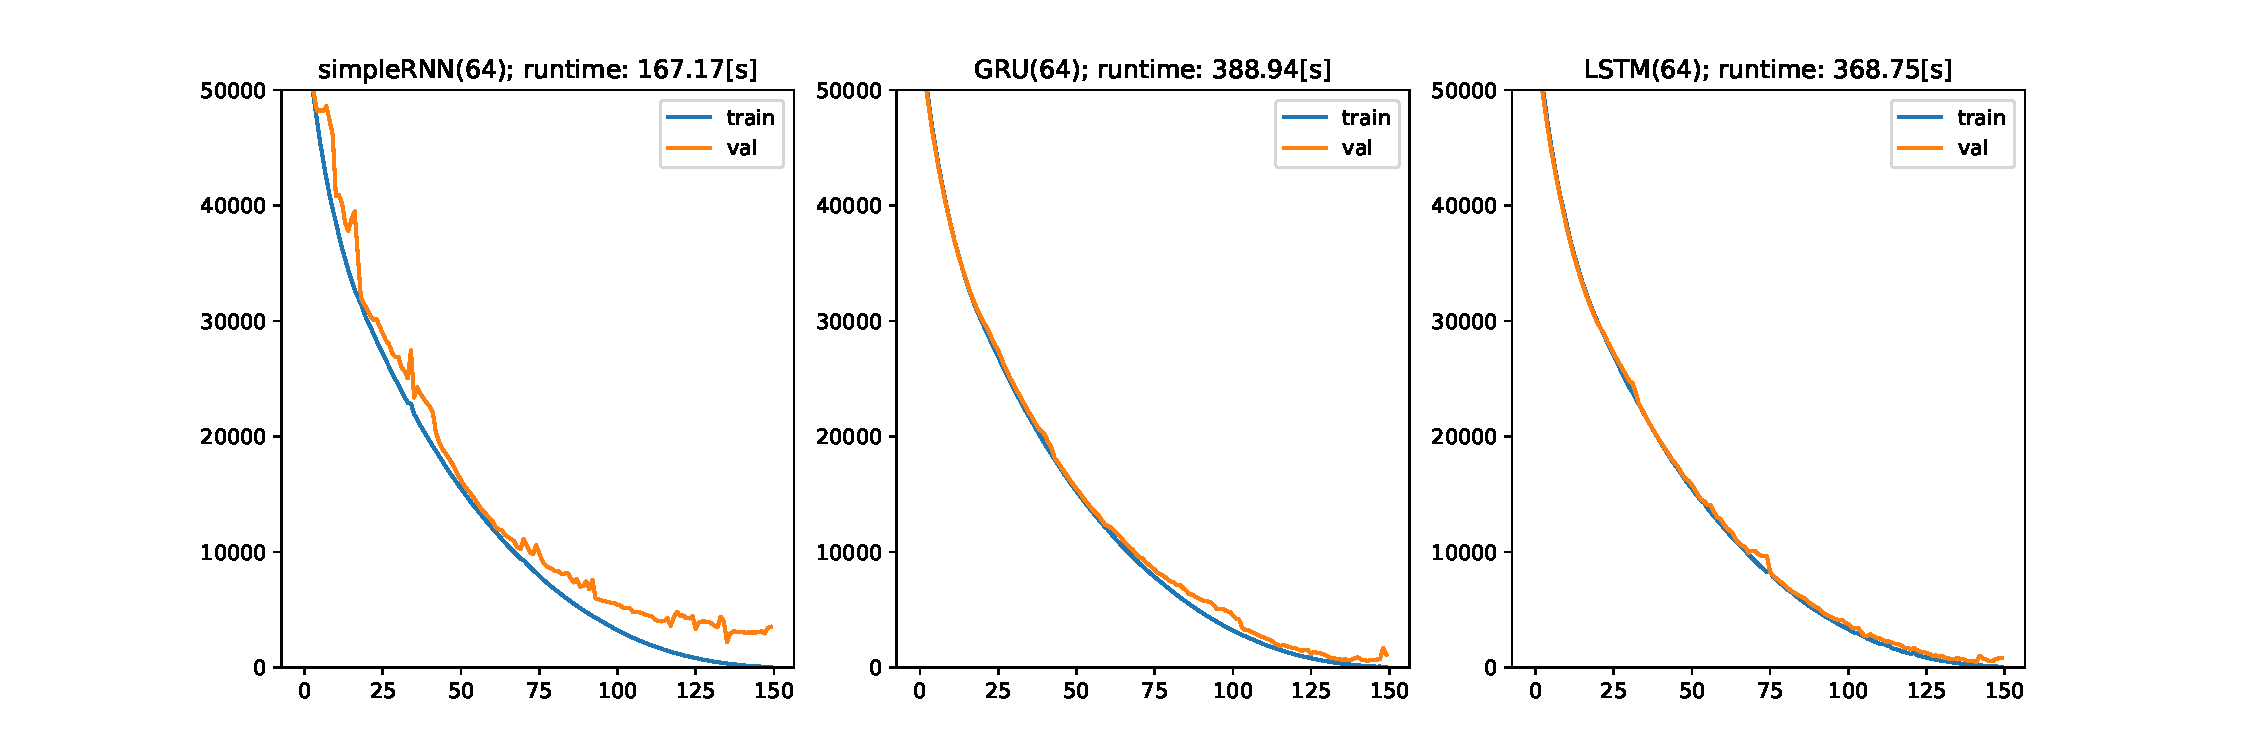
\includegraphics[width = 1\textwidth]{images/compare_models.pdf}
    \caption{Displayed are three different RNN layers as loss functions, trained on the same dataset with the representing runtime in seconds.}
    \label{fig:compare}
\end{figure}
%The \enquote{simpleRNN} loss function in \ref{fig:compare} shows a dispersion between the train and validation indicating overtraining, yet a similar result to the more sufficicated layers. 
%Both \enquote{GRU} and \enquote{LSTM} take approximatly the same time for 150 epochs with similar results. In the following \enquote{SimpleRNN} will be choosen, with \enquote{adam} as an optimizer \cite{keras},
%as the main layer architecture for its short runtime. This first selection has been done with only one layer as a simple representation.
%\subsection{Finetuning SimpleRNN} 
%To apply a fundamental structore to the model a gridsearch, span over an amount of $324$ combinations, will look for the best aoutcome over an epoch count of 150, inlcuding an \enquote{early stop} mechanism with a patience of $10$.
%The gridsearch will search for fititng candidates for: learning rate, units in each layer, layer count, dropout magnitude and batch size. For this each layer represents one layer of SimpleRNN architecture.
\noindent
The \enquote{SimpleRNN} loss function in \ref{fig:compare} shows a dispersion between the train and validation data, indicating overtraining. However, it produces similar results to the more sophisticated layers.
Both \enquote{GRU} and \enquote{LSTM} take approximately the same time for 150 epochs with similar results. In the following, \enquote{SimpleRNN} will be chosen as the main layer architecture for its short runtime, with \enquote{adam} as an optimizer \cite{keras}.
This first selection has been done with only one layer as a simple representation.

\subsection{Finetuning SimpleRNN}
To apply a fundamental structure to the model, a grid search spanning over 324 combinations will look for the best outcome over an epoch count of 150, including an \enquote{early stop} mechanism with a patience of 10.
The grid search will search for fitting candidates for: learning rate, units in each layer, layer count, dropout magnitude, and batch size. For this, each layer represents one layer of SimpleRNN architecture.

\subsection{Gridsearch Results}
\begin{figure}[H]
    \centering
    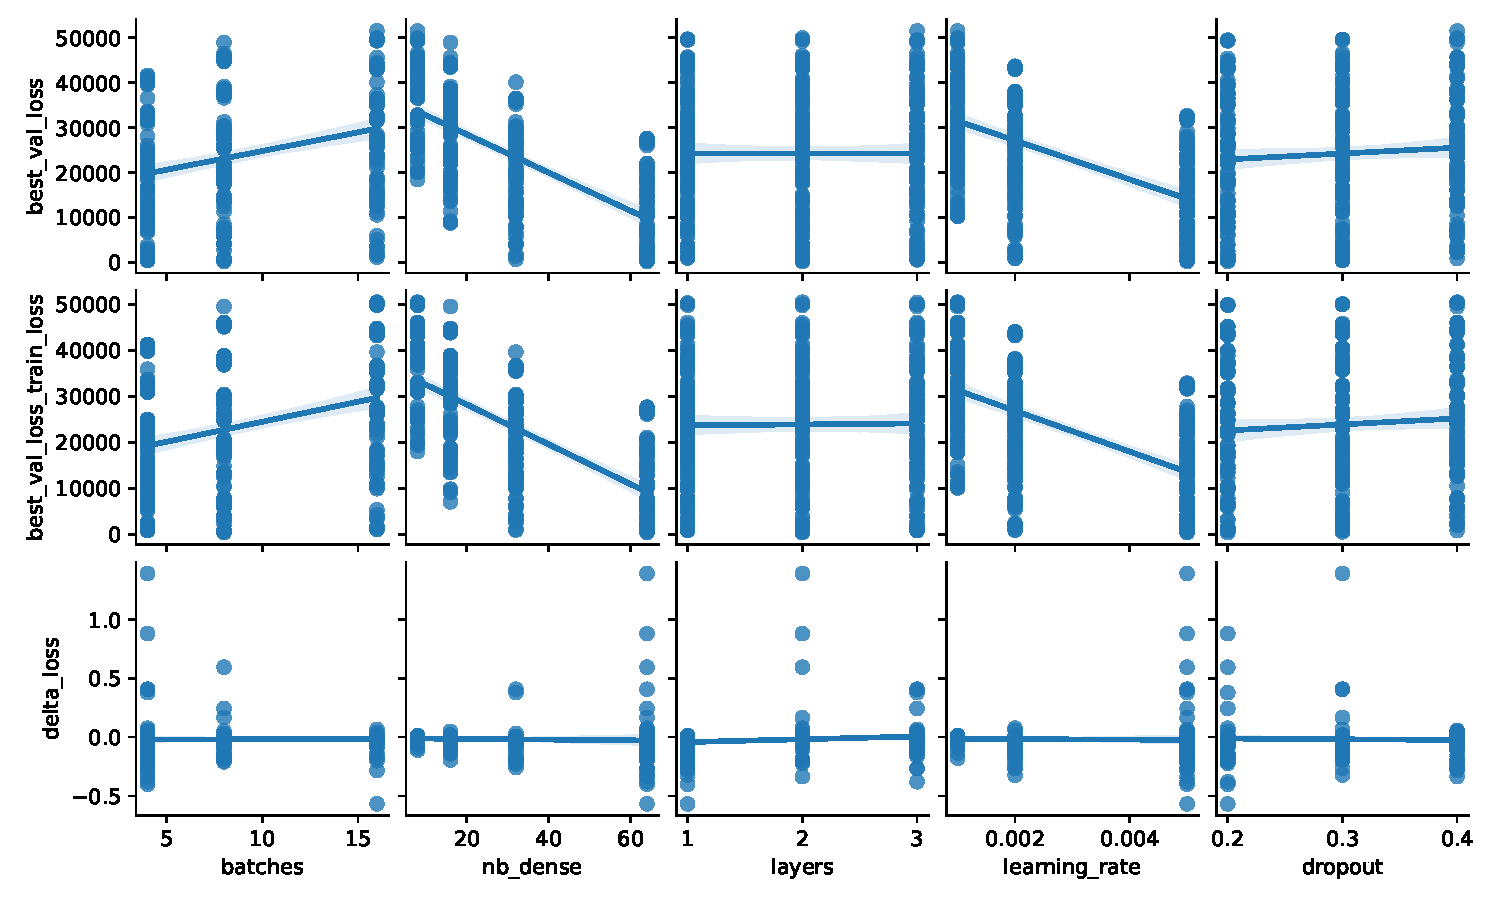
\includegraphics[width = \textwidth]{images/grid_search1.pdf}
    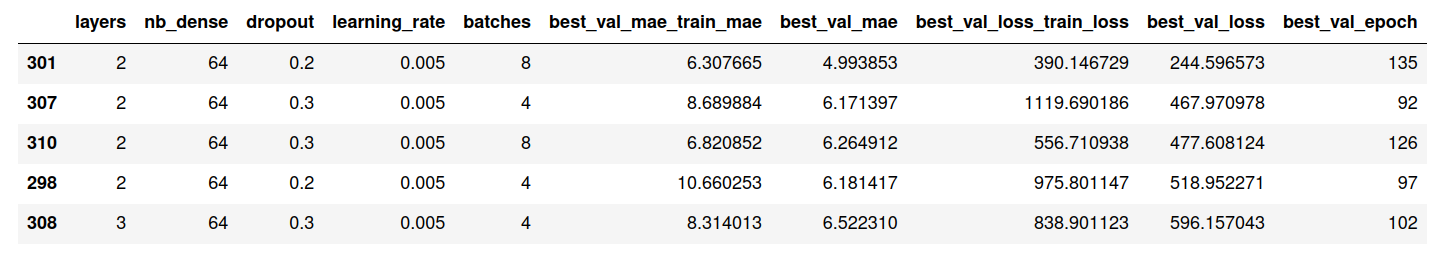
\includegraphics[width = \textwidth]{images/head.png}
    \caption{Displayed is a hyperparameter optimization via gridsearch to find optimal parameters for: learning rate, dropout, numbers of layers and batch size.
            The top graphic displays a \enquote{pairplot} \cite{sns} inlcuding a linear fit to predict the models correlation towards a certain hyperparameter.
            The bottom grahpic shows the first five entries of the presented gridsearch, presenting the found parameters, sorted by \enquote{best\_val\_loss}.}
    \label{fig:grid}
\end{figure}
%The model picked for further finetuning is the third one in the bottom of \ref{fig:grid} since it provides a good validation loss without a big discreptancy towords the training loss which only indicates 
%low overtraining when compared to different models (found by the gridsearch).
%After the application of gridsearch some adjustments will be tried out manually with a focus on the learning rate. 
%For that the optimization learned with a constant rate, a \enquote{learning rate schedualer} will be implemened as a further callbackfunction that automaticly 
%activates himself after a given amount of epochs. The learning rate then decreases in an exponential behaviour, which argument can be further finetuned to acomplish a smooth convergence against the best possible 
%loss rate. For the tuned model an epoch of 100 will be choosen, with an argument of $-0.05$ in the exponential funciton, since from that point the validation loss struggles to converge.
%As the last layer is a dense model with 11 outputs, i.e. the 11 days the model has to predict, a variation of saclers and outputfunctions can be applied. Various scaler do not perform as good as the unsacled 
%target in combination with a \enquote{softplus} activation function, where 
The model picked for further finetuning is the third one at the bottom of \ref{fig:grid}, as it provides a good validation loss without a big discrepancy towards the training loss, indicating only low overtraining compared to different models found by the grid search.
After the application of the grid search, some adjustments will be tried out manually, with a focus on the learning rate. For this purpose, a \enquote{learning rate scheduler} will be implemented as a further callback function that automatically activates itself after a given amount of epochs. The learning rate will then decrease in an exponential manner, and its argument can be further finetuned to achieve a smooth convergence towards the best possible loss rate. For the tuned model, an epoch of 100 will be chosen, with an argument of $-0.05$ in the exponential function, as from that point the validation loss struggles to converge.
As the last layer is a dense model with 11 outputs (i.e., the 11 days the model has to predict), various scalers and output functions can be applied. 
Several scalers do not perform as well as the unscaled target in combination with a \enquote{softplus} \eqref{eq:plus} activation function, where
\begin{equation}
\label{eq:plus}
    \text{softplus}(x) = log(exp(x) + 1) .
\end{equation}

\begin{figure}
\begin{minipage}{0.49\textwidth}
    \centering
    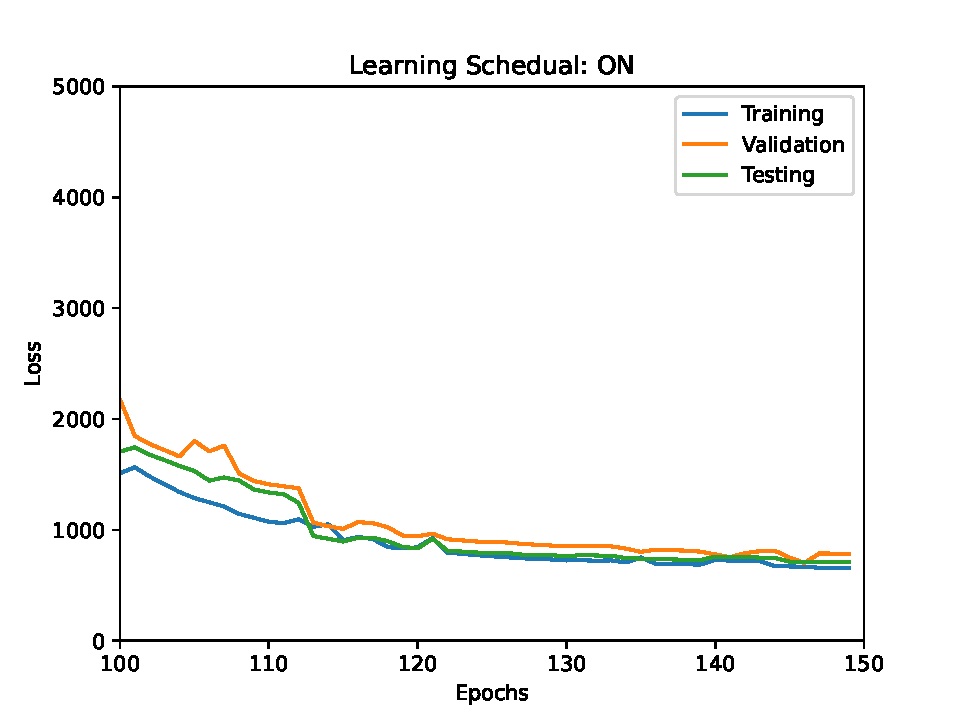
\includegraphics[width = 0.9\textwidth]{images/learning_on.pdf}
\end{minipage}
\begin{minipage}{0.49\textwidth}
    \centering
    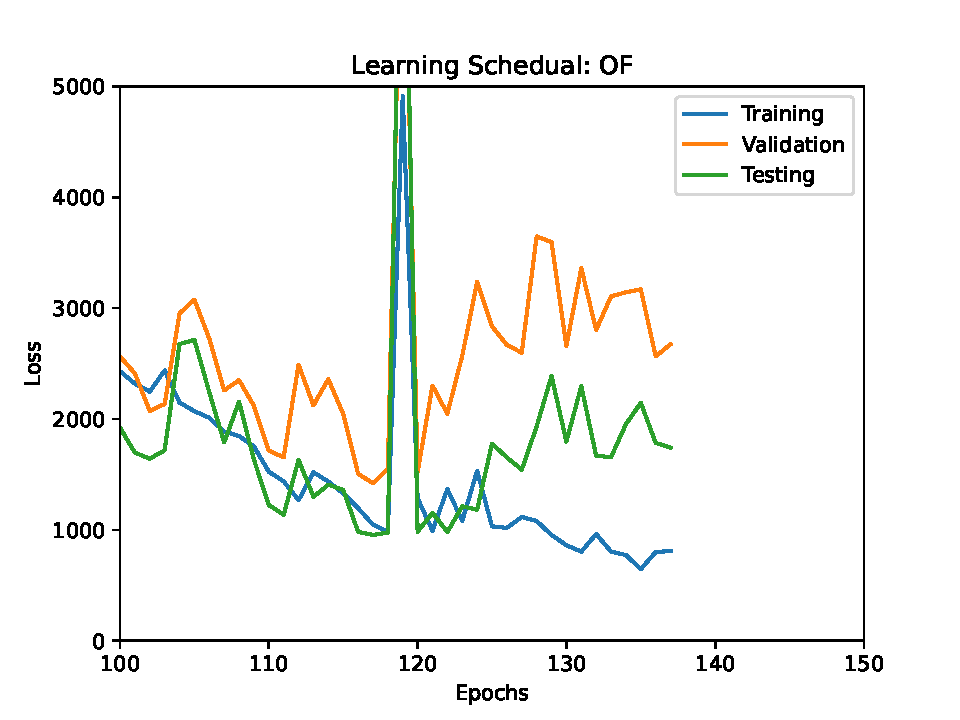
\includegraphics[width = 0.9\textwidth]{images/learning_of.pdf}
\end{minipage}
    \caption{Displayed are two loss curves, both for the same dataset, trained on the same model, but with an activated learning scheduler on the left side. The right side displays the same model without the modified learning rate.}
    \label{fig:loss}
\end{figure}
\noindent
%In \ref{fig:loss} can bee seen how the loss function converges with a dynmic learning rate rather than a constant learning rate where the supposibly local minimum is not found. 
%The same results in the left graphic can also be archieved through lowering the constant learning rate to a certain amount, so the minium will be approached more caregfully, yet this would take more epochs and thus more runtime to acomplish.
%
%\subsection{Keeping Overfitting In Check}
%To avoid overfitting, several mechanism and imported tools will be applied to the model.
%For that it is an indicator of overfitting when the valdiation loss converges yet the tarining loss still decreases, 
%the callbackfunction \enquote{early stop} \cite{keras} will be applied with a patience of $10$ that monitors 
%the validation loss and stops if the current validation loss  will not be undercut after 10 epochs.
%Furthermore for each layer of LSTMs one layer of dropout will force the units to be trained in a general way so that no unit specillizes for the training set.
In \ref{fig:loss}, it can be seen how the loss function converges with a dynamic learning rate rather than a constant learning rate, where the supposedly local minimum is not found. The same results in the left graphic can also be achieved by lowering the constant learning rate to a certain amount, so that the minimum will be approached more carefully. However, this would require more epochs and thus more runtime to accomplish.
\subsection{Keeping Overfitting in Check}
To avoid overfitting, several mechanisms and imported tools will be applied to the model. An indicator of overfitting is when the validation loss converges, yet the training loss still decreases. To address this, the callback function \enquote{early stop} \cite{keras} will be applied with a patience of $10$, which monitors the validation loss and stops training if the current validation loss is not undercut after 10 epochs.
Furthermore, for each layer of SimpleRNNs, one layer of dropout will be added to force the units to be trained in a more generalized way, so that no single unit specializes too much for the training set.